% This chapter to do:
% change figure with cryostat  modifications
% Add TOF and Momentum Plots?

\chapter{LArIAT: Liquid Argon In A Testbeam}\label{sec:experimentDescription}
{\raggedleft ``\emph{But, hey we need to be somewhat foolish...}" \par}
{\raggedleft -- Agnes Obel, 2010 -- \par} %, Avenue,
\vspace{0.5cm}


In this chapter, we describe the LArIAT experimental setup. We start by illustrating the journey of the charged particles in the Fermilab accelerator complex, from the gaseous thermal hydrogen at the Fermilab ion source to the delivery of the LArIAT tertiary beam at MC7. We  then describe the LArIAT beamline detectors, the LArTPC, the DAQ and the monitoring system.

%\section{LArIAT \& the Intensity Frontier}
\section{The Particles' Path to LArIAT}

LArIAT's particle history begins in the Fermilab accelerator complex with a beam of protons. The process of proton acceleration develops in gradual stages (see picture \ref{fig:Accelerator}): gaseous hydrogen is ionized in order to form H$^{-}$ ions; these ions are boosted to 750 keV by a Cockroft-Walton accelerator and injected into the linear accelerator (Linac) that increases their energy up to 400 MeV; then, H$^{-}$ ions pass through a carbon foil and lose the two electrons; the resulting protons are then injected into a rapid cycling synchrotron, called the Booster; at this stage, protons reach 8 GeV of energy and are compacted into bunches; the next stage of acceleration is the Main Injector, a synchrotron which accelerates the bunches up to 120 GeV; in the Main Injector, several bunches are merged into one and are ready for delivery.


The Fermilab accelerator complex works in supercycles of  60 seconds in duration. A 120~GeV primary proton beam with variable intensity is extracted in four-second ``spills" and sent to the Meson Center beam line.  %The beam is split by electrostatic septa and delivered to different experimental halls all over the lab. 

LArIAT's home at Fermilab is the Fermilab Test Beam Facility (FTBF), where the experiment characterizes a beam of charged particles in the Meson Center beam line. 
At FTBF, the primary beam is focused onto a tungsten target to create LArIAT's secondary beam. The secondary beamline is set such that the composition of the secondary particle beam is mainly positive pions. The momentum peak of the secondary beam was fixed at 64~GeV/c for the LArIAT data considered in this work, although the beam is tunable in momentum between 8-80\,GeV/c; this configuration of the secondary beamline assured a stable beam delivery at the LArIAT experimental hall.
 
The secondary beam impinges then on a copper target within a steel collimator inside the LArIAT experimental hall (MC7) to create the LArIAT tertiary beam, (shown in  Fig.~\ref{fig:tert-layout}).   The steel collimator selects particles produced with a $13^\circ$ production angle.   The particles are then bent by roughly $~10^\circ$  through a pair of dipole magnets.  By configuring the field intensity of the magnets we allow the particles of LArIAT's tertiary beam to span a momentum range from 0.2 to 1.4~GeV/c. The polarity of the magnet is also configurable and determines the sign of the beamline particles which are focused on the LArTPC. If the magnet polarity is positive the tertiary beam composition is mostly pions and protons with a small fraction of electrons, muons, and kaons. It is the job of the LArIAT beamline equipment to select the particles polarity,  to perform particle identification in the beamline and to measure the momentum of the tertiary beam particles before they get to the LArTPC. The LArIAT detectors are described in the following paragraphs.  



%\begin{comment}     
\begin{figure}
  \centering  	
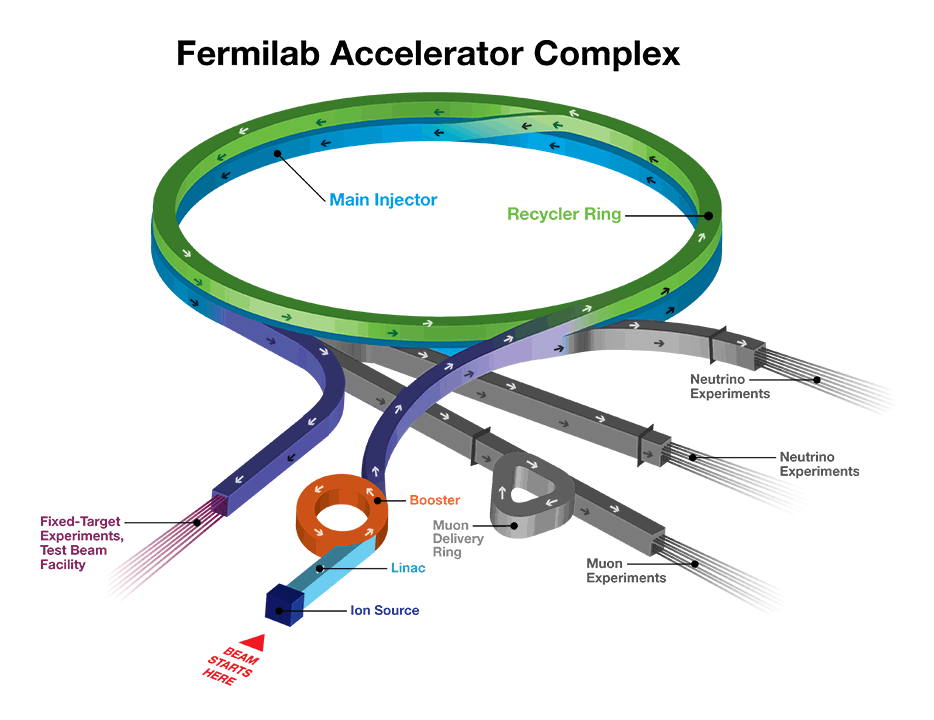
\includegraphics[width=\textwidth,height=\textheight,keepaspectratio]{Chapter-3/Images/AcceleratorFNAL.png}
\caption{Layout of Fermilab Accelerator complex.}
\label{fig:Accelerator}
\end{figure}

%\begin{comment}     
\begin{figure}
  \centering  	
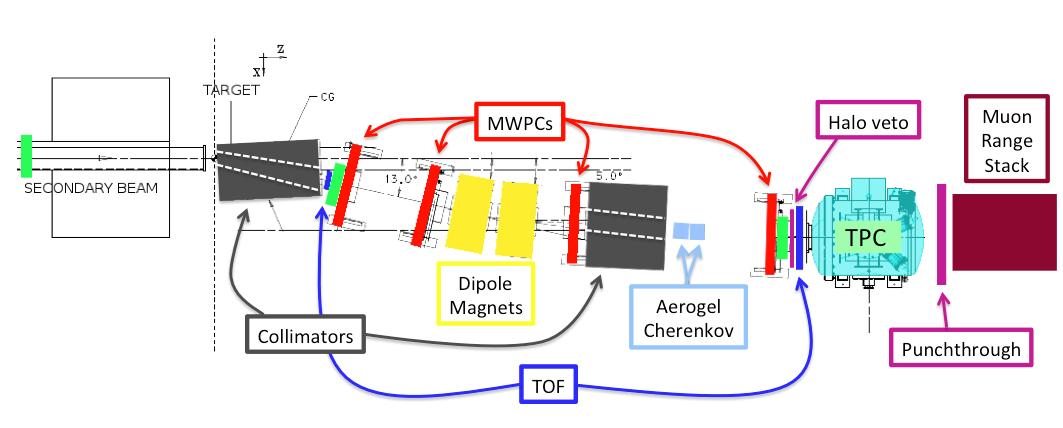
\includegraphics[width=\textwidth,height=\textheight,keepaspectratio]{Chapter-3/Images/Tertiary.png}
\caption{Bird's eye view of the LArIAT tertiary beamline. In grey: upstream and downstream collimators; in yellow: bending magnets; in red: multi wire proportional chambers; in blue: time of flight; in green: liquid argon TPC volume; in maroon: muon range statck.}
\label{fig:tert-layout}
\end{figure}


%%%%%%%%%%%%%%%%%%%%%%%%%%%%%%%%%%%%%%%%%%%%%%%%%%%%%%%%%%%%
\section{LArIAT Tertiary Beam Instrumentation}\label{sec:Instrumentation}

%%%%%%%%%%%%%%%%%%%%%%%%%%%%%%%%%%%%%%%%%%%%%%%%%%%%%%%%%%%%
The instrumentation of the LArIAT tertiary beam and the TPC components have changed several times during the three years of LArIAT data taking. The following paragraphs describe the components operational during ``Run II", the data taking period relevant to the hadron cross section measurements considered in this thesis. 

The key components of the tertiary beamline instrumentation for the hadron cross section analyses are the two bending magnets, a set of four wire chambers (WCs) and two time-of-flight scintillating paddles (TOF) and, of course, the LArTPC.  The magnets determine the polarity of the particles in the tertiary beam; the combination of magnets and wire chambers determines the particles' momenta, which is used to determine the particle species in conjunction with the TOF.
A muon range stack downstream from the TPC and two sets of cosmic paddles configured as a telescope surrounding the TPC are also used for calibration purposes.
A couple of Aerogel Cherenkov counters, which we will not describe here as they are not used in the hadron cross section measurements,  completes the beamline instrumentation.


\subsection{Bending Magnets}\label{sec:Magnets}
%%%%%%%%%%%%%%%%%%%%%%%%%%%%%%%%%%%%%%%%%%%%%%%%%%%%%%%%%%%

LArIAT uses a pair of identical Fermilab type ``NDB" electromagnets, recycled from the Tevatron's anti-proton ring, in a similar configuration used for the  MINERvA T-977 test beam calibration~\cite{MinervaTestbeam}. 
The magnets are a fundamental piece of the LArIAT beamline equipment, as they are used for the selection of the particle polarity and for the momentum measurement before the LArTPC. The sign of the current in the magnets allows us to select either positively or negatively charged particles; the value of the magnetic field is used in the momentum determination and in the subsequent particle identification. 

We describe here the characteristics and response of one magnet, as the second one has a similar response, given its identical shape and history. Each magnet is a box with a rectangular aperture gap in the center to allow for the particle passage.  The magnet aperture measures 14.22~cm in height, 31.75~cm in width, and  46.67~cm in length.  Since the wire chambers aperture ($\sim$12.8~cm$^2$) is smaller than the magnet aperture, only the central part of the magnet gap is utilized. The field is extremely uniform over this limited aperture and was measured with two hall probes, both calibrated with nuclear magnetic resonance probes. The probes measured the excitation curve shown in Figure~\ref{fig:magnet_excitation}. 

\begin{figure}[!h]
\begin{centering}
\vspace{-0.3cm}
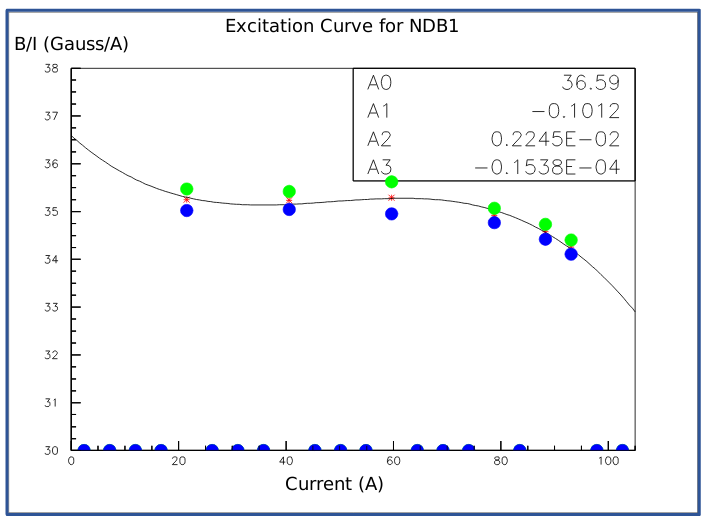
\includegraphics[height=3.0in]{Chapter-3/Images/ExcitationCurves.png}
\caption{
{ Magnetic field over current as a function of the current, for one NDB magnet (excitation curve). The data was collected using two hall probes (blue and green). We fit the readings with a cubic function (black) to average of measurements (red) given in the legend \cite{detectorPaper}.}
}
\label{fig:magnet_excitation}
\end{centering}
\end{figure}

The current through the magnets at a given time is identical in both magnets. For the Run II data taking period, the current settings explored were 60A (B $\sim$0.21 T) and 100A (B $\sim$0.35 T) in both polarities. 
Albeit advantageous to enrich the tertiary beam composition with high mass particles such as kaons, we never pushed the magnets current over 100 A, so as not to incur in overheating.  During operation, we operated an air and water cooling system on the magnets and we remotely monitored the magnet temperatures.
 
\subsection{Multi-Wire Proportional Chambers}\label{sec:MWPC}
%%%%%%%%%%%%%%%%%%%%%%%%%%%%%%%%%%%%%%%%%%%%%%%%%%%%%%%%%%%%
\begin{figure}[!h]
\begin{centering}
\vspace{-0.3cm}
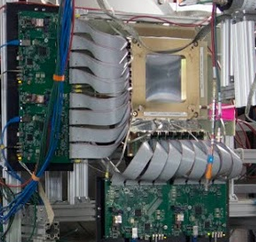
\includegraphics[height=2.3in]{Chapter-3/Images/WireChamber.png}
\caption{
{One of the four Multi Wire Proportional Chambers (WC) used in the LArIAT tertiary beamline and related read-out electronics.}
}
\label{fig:wirechamber}
\end{centering}
\end{figure}

LArIAT uses four multi-wire proportional chambers, or wire chambers (WC) for short, two upstream and two downstream from the bending magnets. The geometry of one chamber is shown in Figure~\ref{fig:wirechamber}: the WC effective aperture is a square of  12.8~cm perpendicular to the beam direction.  Inside the chamber, the 128 horizontal and 128 vertical wires strung at a distance of 1~mm from each other in a mixture of 85\% Argon and 15\% isobutane gas.  The WC operating voltage is between 2400~V and 2500~V. The LArIAT wire chambers are an upgraded version of the Fenker Chambers~\cite{Fenker}, where an extra grounding improves the signal to noise ratio of the electronic readout.  

Two ASDQ chips~\cite{ASDQchip} mounted on a mother board plugged into the chamber serve as front end amplifier/discriminator. The chips are connected to a multi-hit TDC~\cite{Sten} which provides a fast OR output used as first level trigger. The TDC time resolution is 1.18~ns/bin and can accept 2 edges per 9~ns.  
The maximum event rate acceptable by the chamber system is 1 MHz.%: this rate is not a limiting factor considering that the rate of the tertiary particle beam at the first wire chamber is estimated to be less than 15 kHz}. 
A full spill of data occurring once per supercycle is stored on the TDC board memory at once and read out by a specially designed controller.  We use LVDS cables to carry both power and data between the controller and the TDCs and from the controller to the rest of the DAQ.  
%It is possible to program the time window for acceptance for hits, time offsets, front end threshold, and pulse shaping parameters through the controller via a USB from a PC or through an Ethernet connection.

\subsubsection{Multi-Wire Proportional Chambers functionality}\label{sec:MWPCfunc}
We use the wire chamber system together with the bending magnets to measure the particle's momentum.

In the simplest scenario, only one hit on each and every of the four wire chambers is recorded during a single readout of the detector systems.  Thus, we use the hit positions in the two wire chambers upstream of the magnets to form a trajectory before the bend, and the hit positions in the two wire chambers downstream of the magnets to form a trajectory after the bend. We use the angles in the XZ plane between the upstream and downstream trajectories  to calculate the $Z$ component of the momentum as follows:

\begin{equation}
P_z=\frac{B_{eff}L_{eff}}{3.3(sin(\theta_{DS})-sin(\theta_{US}))},
\label{eq:momformula}
\end{equation}

where $B_{eff}$ is the effective maximum field in a square field approximation,  $L_{eff}$ is the effective length of both magnets (twice the effective length of one magnet), $\theta_{US}$ is the angle off the $z$ axis of the upstream trajectory, $\theta_{DS}$ is the angle off the $z$ axis of the downstream trajectory  and  3.3~$c^{-1}$ is the conversion factor from [T$\cdot$m] to [MeV/c]. By using the hit positions on the third and fourth wire chamber, we estimate the azimuthal and polar angles of the particle trajectory, and we are able to calculate the other components of the momentum. 

The presence of multiple hits in a single wire chamber or the absence of hits in one (or more) wire chambers can complicate this simple scenario. The first complication is due to beam pile up, while the latter is due to wire chamber inefficiency. In the case of multiple hits on a single WC, at most one wire chamber track is reconstructed per event. Since the magnets bend particles only in the X direction, we assume the particle trajectory to be roughly constant in the YZ plane, thus we keep the combination of hits which fit best with a straight line. 
It is still possible to reconstruct the particle's momentum  even if the information is missing in either of the two middle wire chambers (WC2 or WC3), by constraining the particle trajectory to cross the plane in between the magnets. 
%Under the assumption of identical magnets, we define a plane centered in the middle of the two magnets (called ``midplane") that the physical particles need to cross. We project the completed half of the wire chamber track to the midplane, assuming no bending, to find the point of intersection. We use this point to complete the other half of the wire chamber track and to calculate the reconstructed momentum  with these four points. To account for the lack of bending in our reconstructed wire chamber track, we apply to the calculated momentum  a correction obtained with a sample of 4-point, single hit tracks.

Events satisfying the simplest scenario of one single hit in each of the four wire chambers form the ``Picky Track" sample.  We construct another, higher statistics sample, where we loosen the requirements on single hit and wire chamber efficiency: the ``High Yield" sample. For LArIAT Run II, the High Yield sample is about three times the Picky Tracks statistics.  
We assume an uncertainty of 2\% for four-point WC track, momentum uncertainty as reported for the same beamline in \cite{MinervaTestbeam}.

%We use Picky Tracks to calibrate the momentum measurement for the High Yield sample, in particular to obtain a momentum correction for  tracks missing information from the central WCs;  this correction adds an uncertainty of approximately 2\% to the momentum calculation of the High Yield sample.




\subsection{Time-of-Flight System}\label{sec:TOF}
%%%%%%%%%%%%%%%%%%%%%%%%%%%%%%%%%%%%%%%%%%%%%%%%%%%%%%%%%%%%
Two scintillator paddles, one upstream of the first set of WCs and one downstream of the second set of WCs  form LArIAT  time-of-flight (TOF) detector system. 

The upstream paddle is made of a 10 x 6 x 1~cm scintillator piece, read out by two PMTs mounted on the beam left side which collect the light from light guides mounted on all four edges of the scintillator. The downstream paddle is a   14 x 14 x 1~cm scintillator piece read out by two PMTs on the opposite ends of the scintillator, as shown in figure \ref{fig:TOF}.
The relatively thin width in the beamline direction minimizes energy loss of beam particles traveling through the scintillator material.

The CAEN 1751 digitizer is used to digitize the TOF PMTs signals at a sampling rate of 1 GHz. The 12 bit samples are stored in a circular memory buffer. At trigger time, data from the TOF PMTs are recorded to output in a 28.7 \textmu s windows starting  approximately 8.4 \textmu s before the trigger time. 


\subsubsection{TOF functionality}\label{sec:TOFfunc}


The TOF signals rise time (10-90\%) is 4 ns and a full width, half-maximum of 9 ns consistent in time. The signal amplitudes from the upstream TOF and  downstream TOF are slightly different:  200 mV for the upstream PMTs but only 50 mV for downstream PMTs. The time of the pulses was calculated utilizing an oversampled template derived from the data itself. We take the pulse pedestal from samples far from the pulse and subtract it from the pulse amplitude. We then vertically stretch  a template to match the pedestal-subtracted pulse amplitude and we move it horizontally to find the time. With this technique, we find a pulse time-pickoff resolution better than 100 ps.  The pulse pile up is not a significant problem given the TOF timing resolution and the rate of the particle beam.  Leveraging on the pulses width uniformity of any given PMT,  we flag events where two pulses overlap as closely in time as 4 ns with a 90\% efficiency according to simulation. 


We combine the pulses from the two PMTs on each paddle to determine the particles' arrival time by averaging the time measured from the single PMT, so to minimize errors due to optical path differences in the scintillator.  However, a time spread of approximately 300~ps is present in both the upstream and downstream detectors, likely due to transit time jitter in the PMTs themselves.  %There is no evidence of systematic timing drift over long data-taking periods such as 3-4 months: the maximum variation of the average time differences between pairs of PMTs reading out the same scintillator is of the order of 150~ps.

\begin{figure}[h!]
\centering
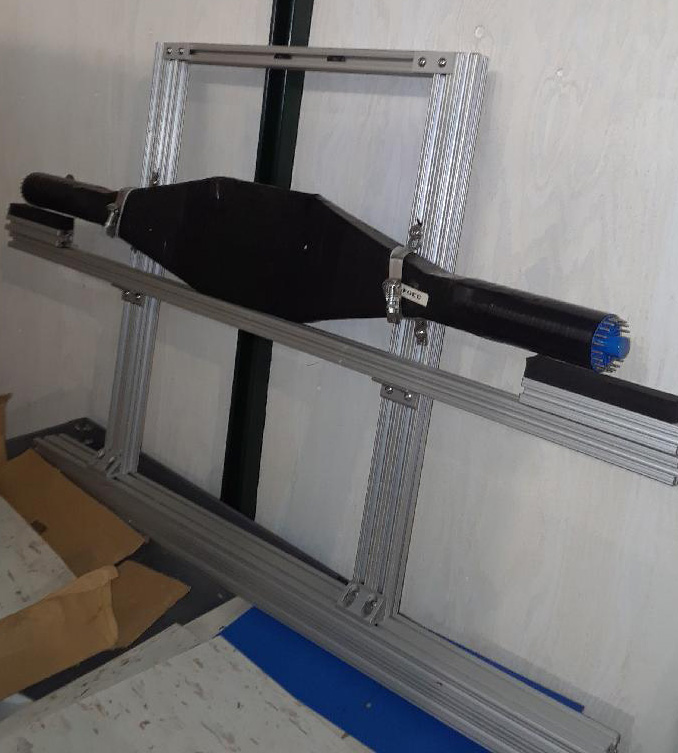
\includegraphics[width=0.5\textwidth]{Chapter-3/Images/DSTOF.jpg}
\caption{Image of the down stream time of flight paddle, PMTs and relative support structure before mounting. } 
\label{fig:TOF}
\end{figure}


%\textcolor{red}{calculated TOF with error}


%%%%%%%%%%%%%%%%%%%%%%%%%%%%%%%%%%%%%%%%%%%%%%%%%%%%%%%%%%%%
\subsection{Punch-Through and Muon Range Stack Instruments}\label{sec:MuRS}
%%%%%%%%%%%%%%%%%%%%%%%%%%%%%%%%%%%%%%%%%%%%%%%%%%%%%%%%%%%%

The punch-through and the muon range stack (MuRS) detectors are located downstream of the TPC. These detectors provide a sample of  TPC crossing tracks without relying on TPC information and can be used to improve particle ID for  muons and pions with momentum higher than  450 MeV/c.

The punch-through is simple sheet of scintillator material, read out by two PMTs. 
The MuRS is a segmented block of steel with four slots instrumented with scintillation bars. The four steel layers in front of each instrumented slot are 2 cm, 2 cm, 14 cm and 16 cm deep in the beam direction. Each instrumented slot is equipped with four scintillation bars each, positioned horizontally in the direction orthogonal to the beam. Each scintillator is read out by one PMT.  

The signals from both the punch-thorough and the MuRS PMTs  are sent to a NIM discriminator. If the signal crosses the discriminator threshold, it is digitized in the CAEN V1740, same as the TPC. The sampling time of the CAEN V1740 is slow (of the order of 128 ns) and that the pulse shape information from the PMT is lost. A Punch-thorough and MuRS signal will then be simply a ``hit" at a given time in the beamline event.


It is worth mentioning here the presence of an additional scintillation paddle between WC4 and the downstream paddle of the TOF system, called halo. The halo is a 39 x 38 x 1 cm$^3$ paddle with a 6.5 cm radius hole in the center, whose original function was to reject  beam particles slightly offset from the beamline center. Data from this paddle turned out to be unusable, so our data events include both particle going through the halo scintillation material or through the halo hole.

%%%%%%%%%%%%%%%%%%%%%%%%%%%%%%%%%%%%%%%%%%%%%%%%%%%%%%%%%%%%
\subsection{LArIAT Cosmic Ray Paddle Detectors}\label{sec:CosmicRayPaddle}
%%%%%%%%%%%%%%%%%%%%%%%%%%%%%%%%%%%%%%%%%%%%%%%%%%%%%%%%%%%%
LArIAT triggers both on beam events and on cosmic rays events. We perform this latter trigger by using two sets of cosmic ray paddle detectors (a.k.a. ``cosmic towers".) The cosmic towers frame the LArIAT cryostat, as one sits in the downstream left corner and the other sits in the upstream right corner of the cryostat. Two paddle sets of four scintillators pieces each make up each cosmic tower, an upper set and a lower set per tower. 
Of the four paddles, a couple of two matched paddles stands upright while the a second matched pair lies across the top of the assembly in the top sets (or across the bottom of the assembly in the bottom sets). The horizontal couple is used as a veto for particles traveling from inside the TPC out.  The four signals  from the vertical paddles along one of the body diagonals of the TPC are combined in a logical ``AND''. This allows to select track due to cosmic muons at the ground level crossing the TPC along one of its diagonals.  Cosmic ray muons whose average energy is in the few GeV range crossing both anode and cathode populate the events triggered this way. This particularly useful sample of tracks is associated can be used for many tasks; for example, we use anode-cathode piercing tracks to cross check the TPC electric field on data (see Appendix \ref{ch:AppendixB}), to calibrate the charge response of the TPC wires for the full TPC volume and to measure the electron lifetime in the chamber \cite{LArIATLifeTime}.

%%%%%%%%%%%%%%%%%%%%%%%%%%%%%%%%%%%%
%All the paddles are 3.02~cm thick and are  trapezoidal in shape. The paddles come in two sizes: the smaller version has bases 32.2~cm and 26.7~cm, and 61.0~cm height, while the bigger version has bases 33.2~cm and 27.0~cm, and $70.8~cm$ height. 
% A Zener-diode Hamamatsu H5783 PMT collects the light from a wavelength-shifting optical fiber which runs along one of the long sides of each paddle. A custom-made PMT Amplifier and Discrimination (PAD) circuit mounted at one end of the paddle collects signals from the PMTs and sends them to the Control and Concentrator Unit (CCU). We use the same connection to  power the PMT, control voltage and threshold, and output the PMT signal as logic ECL pulse.
We retrieved the scintillation paddles from the decommissioning of the CDF detector at Fermilab and we used only the paddles with a counting efficiency greater than 95\% and low noise at working voltage. The measured trigger rate of the whole system is 0.032~Hz, corresponding to $\sim 2$ muons per minute.


\begin{figure}[h!]
\centering
 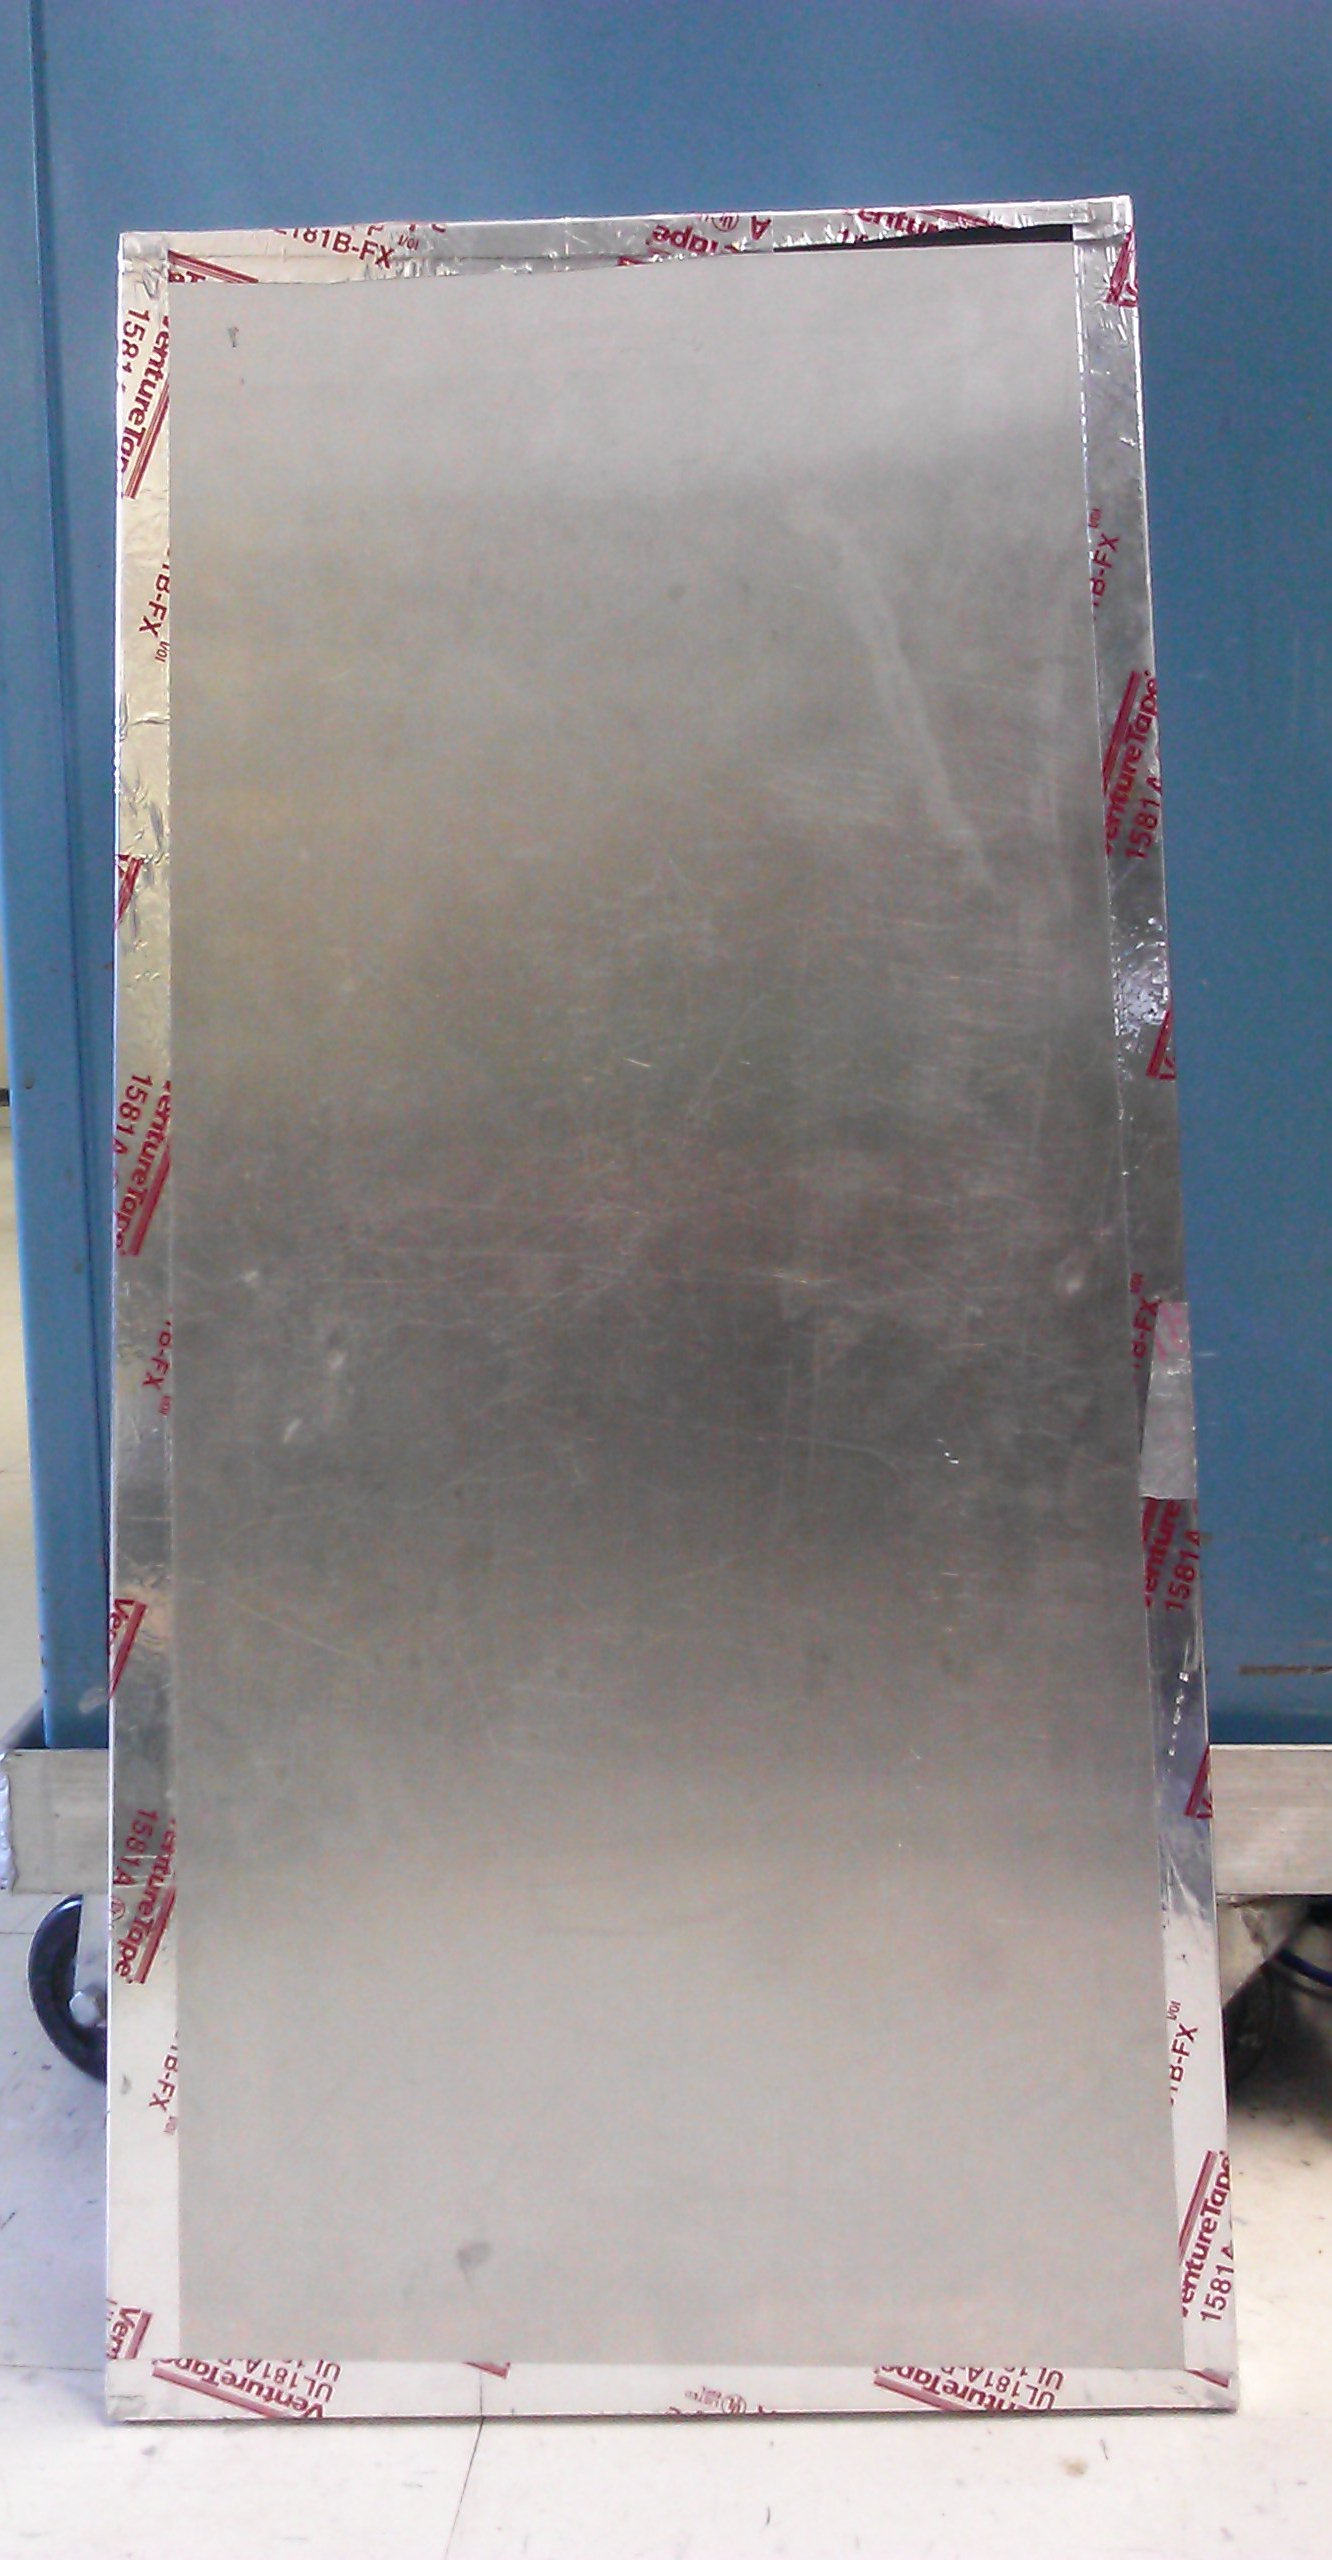
\includegraphics[angle=90,width=0.7\textwidth]{Chapter-3/Images/Cosmic_Paddle.jpg}
\caption{Photograph of one of the scintillation counters used in the cosmic towers. } 
\label{pic:cosmicpaddle}
\end{figure}





\section{In the Cryostat}
The heart of the LArIAT experiment lives in the LArIAT cryostat. In this section, we describe the cryogenic system and the argon purity (Section \ref{ch:Cryo}), the LArIAT TPC (Section \ref{sec:TPCCharge}) and light collection system (\ref{sec:TPCLight}).
\subsection{Cryogenics and Argon Purity}\label{ch:Cryo}
LArIAT repurposed the ArgoNeuT cryostat \cite{ArgoNeuT-det} in order to use it in a beam of charged particles, and added a new process piping and a new liquid argon filtration system in FTBF.  %The main modifications to the ArgoNeuT cryostat are the addition of a beam flange and a port for the light collection system, 
Inside the LArIAT experimental hall, the cryostat sits in the beam of charged particles with its horizontal main axis oriented parallel to the secondary beam, ~3$^\circ$ off axis from the tertiary beam

Two volumes make up LArIAT cryostat, shown in Figure \ref{fig:LArIATCryoStat}:  the inner vessel and the outer vessel. Purified liquid argon fills the inner vessel, while the outer volume provides insulation through a vacuum jacket equipped with layers of aluminized mylar superinsulation. The inner vessel is a cylinder of 130~cm length and 76.2~cm diameter, containing about 550~L of LAr, corresponding to a mass of 0.77 ton. We run the signal cables for the LArTPC and the high voltage feedthrough through a ``chimney'' at the top and mid-length of the cryostat.


\begin{figure}[htb]
\centering
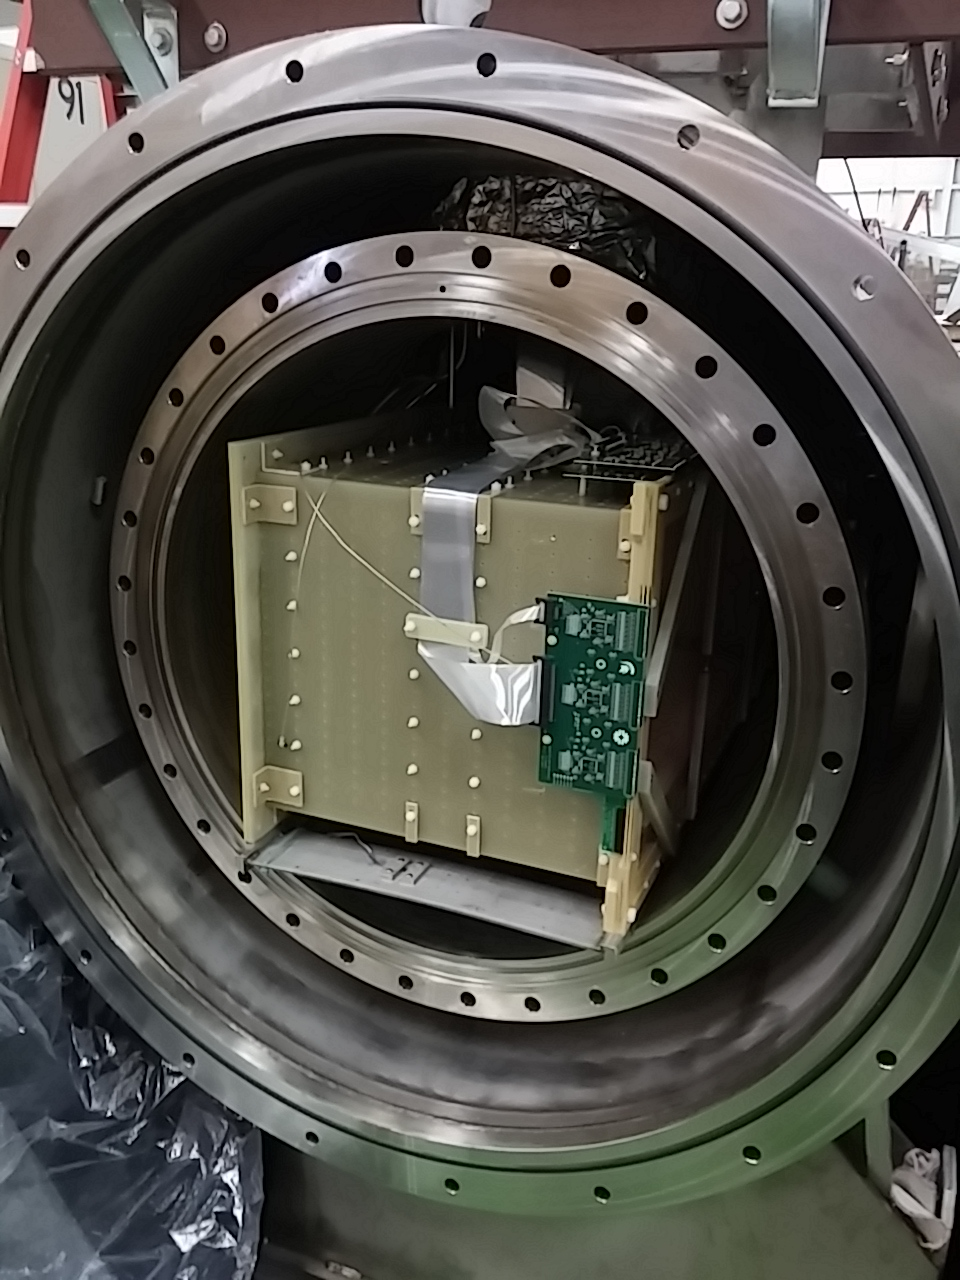
\includegraphics[scale=0.18]{Chapter-3/Images/Cryostat1.jpg}
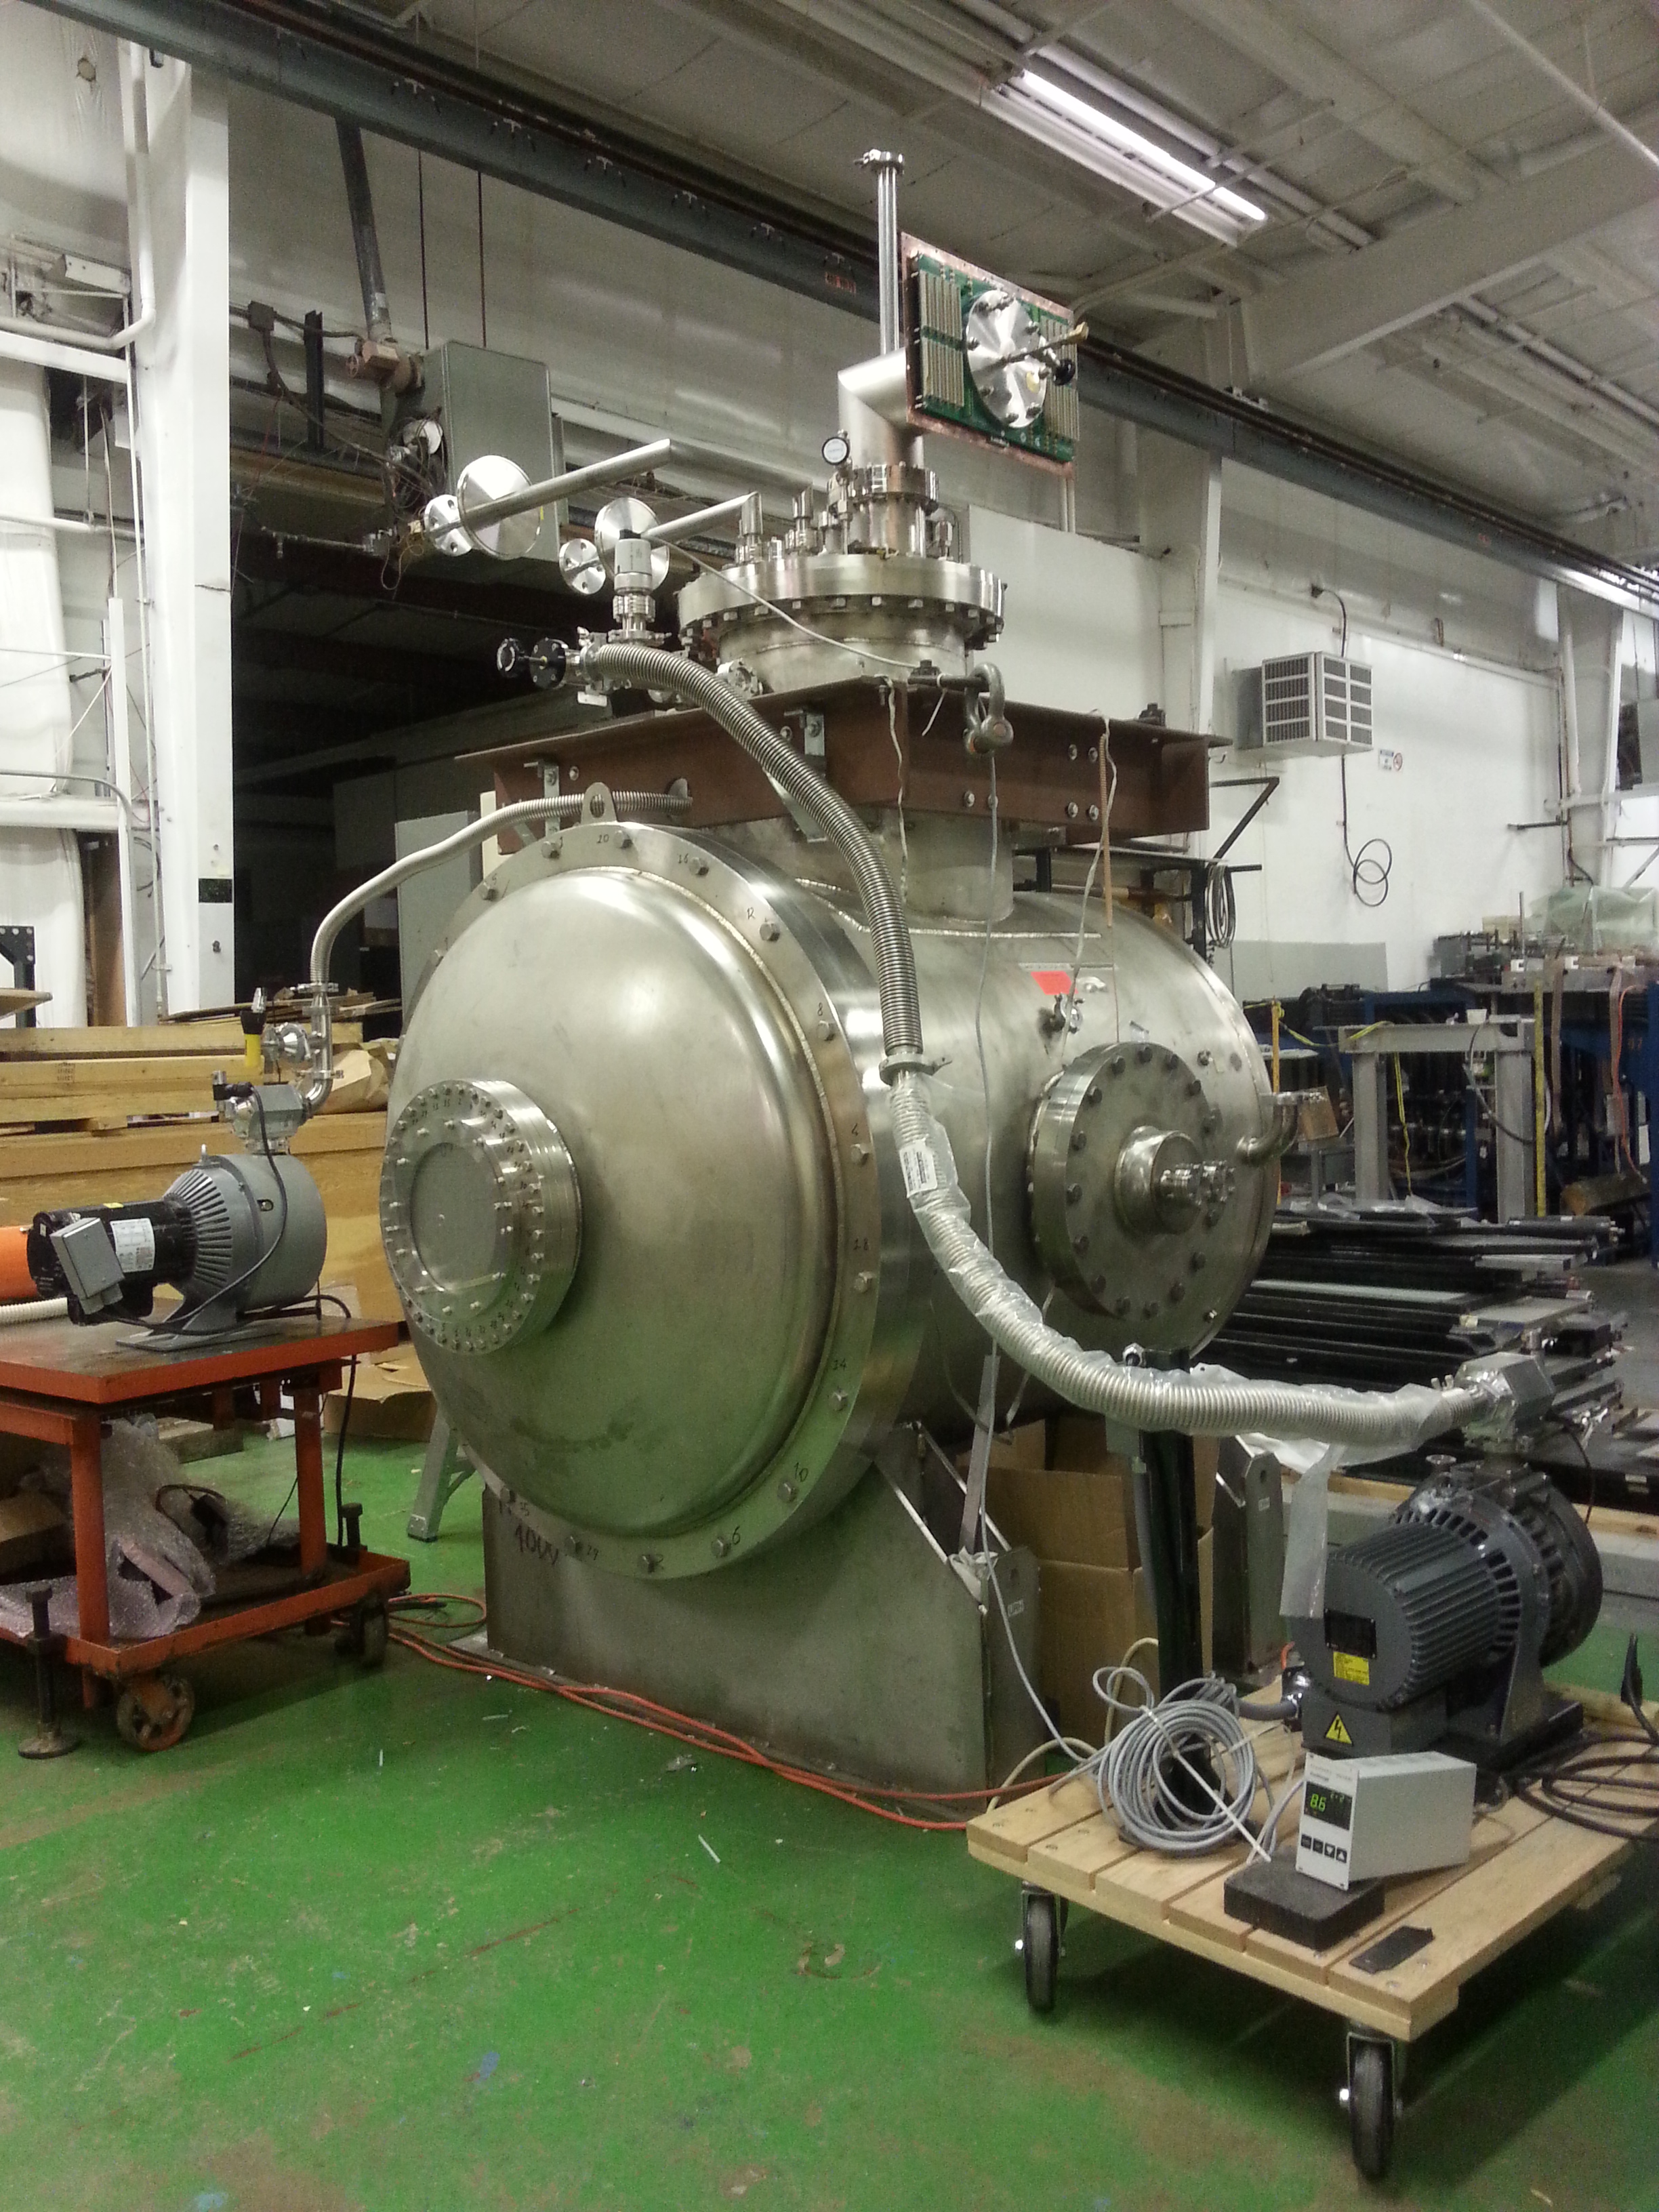
\includegraphics[scale=0.07]{Chapter-3/Images/Cryostat2.jpg}
\caption{ Left: the LArIAT TPC in the inner volume of the open cryostat. Right: cryostat fully sealed ready to be transported to FTBF. }
\label{fig:LArIATCryoStat}
\end{figure}

Given the different scopes of the ArgoNeuT and LArIAT detectors, we made several modifications to the ArgoNeuT cryostat in order to use it in LArIAT. In particular, the modifications  shown in Figure \ref{fig:LArIATCryoMods} were necessary to account for the beam of charged particles entering the TPC and to employ the new FTBF liquid argon purification system. 
We added a ``beam window'' on the front outer end cap and an ``excluder'' on the inner endcap, with the purpose of minimizing the amount of non-instrumented material upstream of the TPC's active volume. The amount of non-instrumented material in front of the TPC for LArIAT corresponds to $\sim$0.3 electron radiation lengths ($X_{0}$), to compare against the  $\sim 1.6 X_{0}$ of ArgoNeuT. To allow studies of the scintillation light, we added a side port feedthrough which enables the mounting of the light collection system, as well as the connections for the corresponding signal and high-voltage cables (see Section \ref{sec:TPCLight}).  We modified the bottom of the cryostat adding Conflat and ISO flange sealing to connect the liquid argon transfer line to the new argon cooling and purification system.


\begin{figure}[htb]
\centering
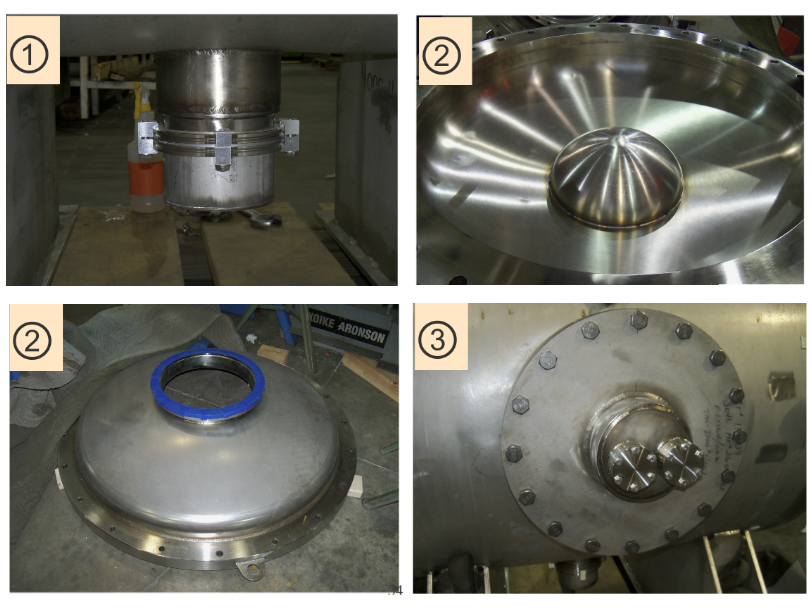
\includegraphics[scale=0.35]{Chapter-3/Images/CryoMods.png}
\caption{Main modifications to the ArgoNeuT cryostat: $1)$ outlet for connection to the purification system at the bottom of the cryostat; $2)$ the ``beam-window'' on the outer endcap and ``excluder"  which reduces the amount of non-instrumented material before the TPC; $3)$ the side port to host  the  light collection system.}
\label{fig:LArIATCryoMods}
\end{figure}

%%%%%%%%%%%%%%%%%%%%%
As in any other LArTPC, argon purity is a crucial parameter for LArIAT. Indeed, the presence of contaminants affects both the basic working principles of a LArTPC, as shown in Section \ref{sec:LArTPCWorkingPrinciple}: electronegative contaminants such as oxygen and water decrease the number of ionization electrons collected on the wires after drifting through the volume. In addition, contaminants such as Nitrogen decrease the light yield from scintillation light, especially in its slow component.
In LArIAT, contaminations should not exceed the level of 0.2 parts per billion (ppb). We achieve this level of purity in several stages. The specifics required for the commercial argon bought for LArIAT are 2 parts per million (ppm) oxygen, 3.5~ppm water, and 10~ppm nitrogen. This argon is monitored with the use of commercial gas analyzer.
Argon is stored in a dewar external to LArIAT hall and filtered before filling the TPC. %The argon is delivered from the commercial dewar to the cryostat through 2.54~cm diameter schedule 10 stainless steel piping.  The piping was insulated with 20.32~cm of polyurethane foam by the manufacturer.  The piping was cleaned to remove oil and grease before being welded into the system. 
LArIAT uses a filtration system designed for the Liquid Argon Purity Demonstrator (LAPD)~\cite{LAPD}: half of a 77~liter filter contains a 4A molecular sieve (Sigma-Aldrich~\cite{sigma-aldrich}) able to remove mainly water, while the other half contains BASF~CU-0226~S, a highly dispersed copper oxide impregnated on a high surface area alumina, apt to remove mainly oxygen~\cite{basf}. A single pass of argon in the filter is sufficient to achieve the necessary purity, unless the filter is saturated. In case the filter saturates, the media needs to be regenerated by using heated gas; this happened twice during the Run II period\footnote{We deemed the filter regeneration necessary every time the electron lifetime dropped under 100 \textmu s.}. The electron lifetime during the full LArIAT data taking are shown in Figure \ref{fig:Elifetime}.
The filtered argon reaches the inner vessel via a liquid feedthrough which is routed to the bottom of the cryostat. Argon is not recirculated in the system; rather, it boils off and vents to the atmosphere. During data taking, we replenish the argon in the cryostat every 6 hours to keep the TPC high voltage feedthrough and cold electronics always submerged. In fact, we constantly monitor the level, temperature, and pressure of the argon both in the commercial dewar and inside the cryostat during data taking. 
\subsection{LArTPC: Charge Collection}\label{sec:TPCCharge}
The LArIAT Liquid Argon Time Projection Chamber is a rectangular box of dimensions 47 cm (drift) x 40 cm (height) x 90 cm (length), containing 170 liters of Liquid Argon.
The LArTPC three major subcomponents are 
\begin{itemize} 
\item[1)] the cathode and field cage,
\item [2)] the wire planes, 
\item [3)] the read-out electronics. %
\end{itemize}





\subsubsection{Cathode and field cage}
A G10 plain sheet with copper metallization on one of the 40 x 90~cm inner surfaces forms the cathode. 
A high-voltage feedthrough on the top of the LArIAT cryostat delivers the high voltage to the cathode; the purpose of the high voltage system (Figure~\ref{fig:HVScheme}) is to drift ionization electrons from the interaction of charged particles in the liquid argon to the wire planes.  The power supply used in this system is a Glassman LX125N16 ~\cite{GlassmanPS} capable of generating up to -125~kV and 16~mA of current, but operated at -23.5kV during LArIAT Run-II. The power supply is connected via high voltage cables to a series of filter pots before finally reaching the cathode. 

\begin{figure}[htb]
\centering
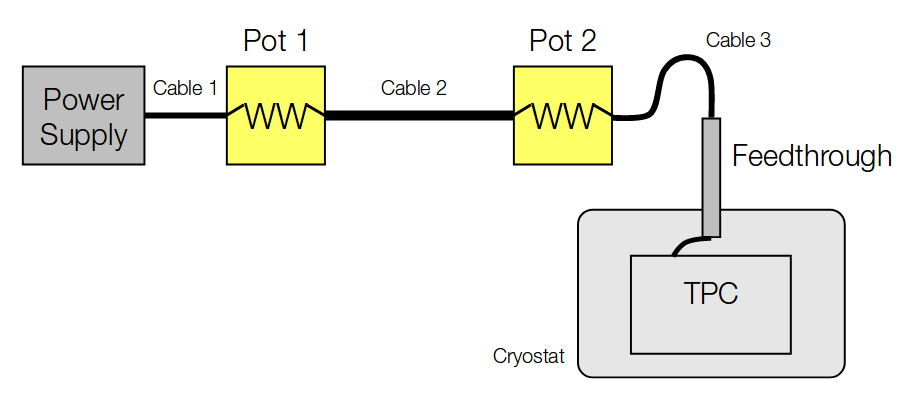
\includegraphics[scale=0.35]{Chapter-3/Images//HVSchematic.png}\\
\caption{Schematic of the LArIAT high voltage system.}
\label{fig:HVScheme}
\end{figure}%See DocDB 1472



The field cage is made of twenty-three parallel copper rings framing the inner walls of the G10 TPC structure. A network of voltage-dividing resistors connected to the field cage rings steps down the high voltage from the cathode to form a uniform electric field. The electric field over the entire TPC drift volume is  486 V/cm, as measured in appendix \ref{ch:AppendixB}. The  maximum drift length, i.e. the distance between cathode and anode planes, is 47 cm.

\subsubsection{Wire planes}
LArIAT Run-II has three wire planes separated by 4 mm spaces: in order of increasing distance from the cathode, they are the shield, the induction and the collection plane. The ``wire pitch", i.e., the distance between two adjacent wires in a given plane, is 4 mm.  The shield plane counts 225 parallel wires of equal length oriented vertically. This plane is not connected with the read-out electronics; rather it shields the outer planes from extremely long induction signals due to the ionization in the whole drift volume. As the shield plane acts almost like a Faraday cage, the resulting shape of signals in the first instrumented plane (induction) is easier to reconstruct.  Both the induction and collection planes count 240 parallel wires of different length oriented at 60$^\circ$ from the vertical with opposite signs.
Electrons moving past the induction plane will induce a bipolar pulse on its wires; the drifting electrons will be then collected on the collection plane's wires, forming a unipolar pulse. 

The three wire planes and the cathode form three drift volumes, as shown in Figure \ref{fig:driftregions}. 
The main drift volume is defined as the region between the cathode plane and the shield plane (C-S). The other two drift regions are those between the shield plane and the induction plane (S-I), and between the induction plane and the collection plane (I-C). The electric field in these regions is chosen to satisfy the charge transparency condition  and allow for 100$\%$ transmission of the drifting electrons through the shield and the induction planes; for example, the transparency condition between for the shield plane reads
\begin{equation}
\frac{E_{S-I}}{E_{C-S}} > \frac{1+\rho}{1-\rho},
\end{equation}
where $E_{C-S}$ is the electric field in the region between the cathode and the shield plane, $E_{S-I}$ is the electric field in the region between the shield and the induction plane, and $\rho = \frac{2\pi \text{ }r}{D}$ is a factor accounting for the radius of the wires $r$ (152 $\mu m$) and the gap distance $D$ (4 mm). An analogous condition can be written for the induction plane.
\begin{figure}[htb]
\centering
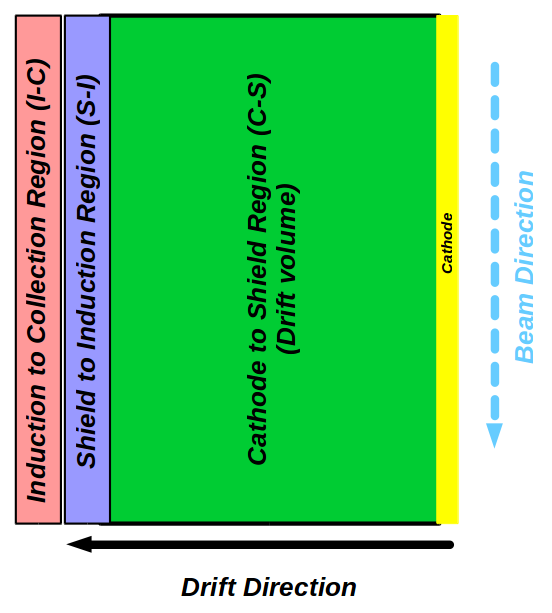
\includegraphics[scale=0.35]{Chapter-3/Images/DriftRegions.png}\\
\caption{Schematic of the three drift regions inside the LArIAT TPC: the main drift volume between the cathode and the shield plane (C-S) in green, the region between the shield plane and the induction plane (S-I) in purple, and the region between the induction plane and the collection plane (I-C) in pink.}
\label{fig:driftregions}
\end{figure}

Table \ref{tab:voltages} provides the default voltages applied to the cathode and the shield, induction, and collection plane.  

\begin{table}[htpb]
\centering
\caption{Cathode and anode planes default voltages}
\label{tab:voltages}
\begin{tabular}{llll}
\hline
\multicolumn{1}{|l|}{ Cathode} & 
\multicolumn{1}{|l|}{ Shield} & \multicolumn{1}{l|}{ Induction} & \multicolumn{1}{l|}{ Collection}  \\ \hline
\multicolumn{1}{|l|}{-23.17 kV} &
\multicolumn{1}{|l|}{-298.8 V} & \multicolumn{1}{l|}{-18.5 V}      & \multicolumn{1}{l|}{338.5 V} \\ \hline
\end{tabular}
\end{table}


\subsubsection{Electronics}

Dedicated electronics read the induction and collection plane wires, for a total of  480-channel analog signal path from the TPC wires to the signal digitizers. A digital control system for the TPC-mounted electronics, a power supply, and a distribution system complete the front-end system. Figure \ref{pic:FEelectronics} shows a block diagram of the overall system. The direct readout of the ionization electrons in liquid argon forms typically small signals on the wires, which need amplification in oder to be processed. LArIAT  performs the amplification stage directly in cold with  amplifiers %developed by the Brookhaven National Lab (BNL) and 
mounted on the TPC frame inside the liquid argon. The BNL ASICs adopted in LArIAT are designated as LArASIC, version 4-star and are the same used by the MicroBooNE experiment \cite{Acciarri2017}.
%The ASIC signals for each wire are then driven out of the vessel  to DAQ boards that act as waveform recorders.
The signal from the ASICs are driven to the other end of the readout chain, to the CAEN V1740 digitizers \cite{CAENV1740}. The CAEN V1740 has a 12 bit resolution and a maximum input range of 2~VDC, resulting in about 180 ADC count for a crossing MIP.   

\begin{figure}[htbp]
 \centering
 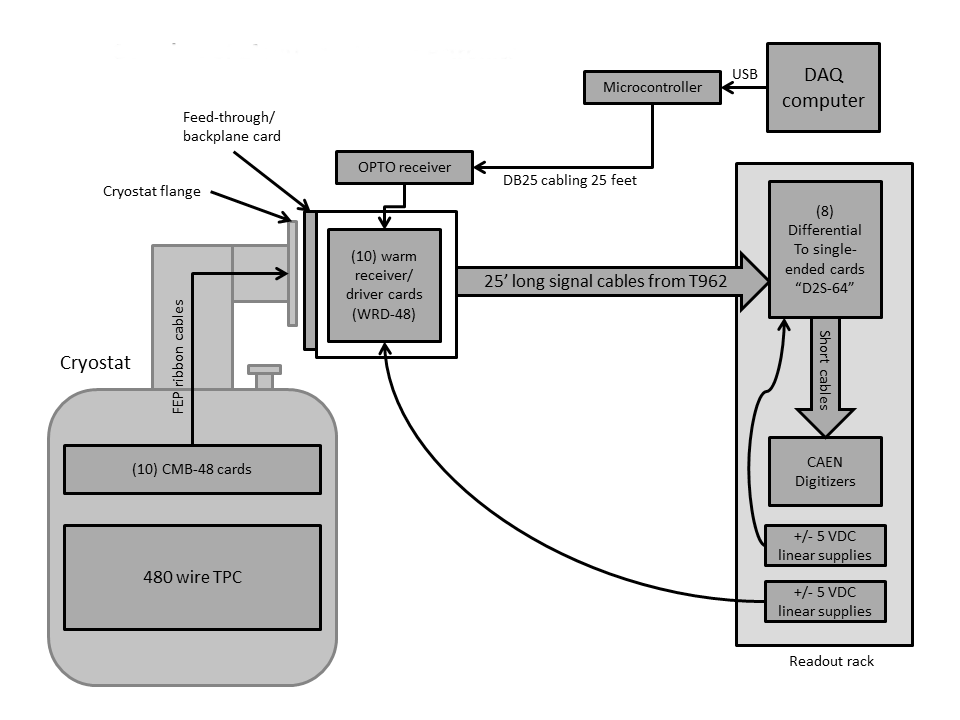
\includegraphics[width=1.0\textwidth]{Chapter-3/Images/LArIAT_FE_Electronics.png}
\caption{Overview of LArIAT Front End electronics. } 
\label{pic:FEelectronics}
\end{figure}




\subsection{LArTPC: Light Collection System}\label{sec:TPCLight} 
The collection of scintillation photons is the second mechanism of particle detection in argon other than the ionization electrons. Over the course of LArIAT's three years of data taking, the light collection system changed several times. We describe here the light collection system for Run II. Two PMTs, a 3-inch diameter Hamamatsu R-11065 and 2-inch diameter ETL D757KFL~\cite{lightsys-pmttests}, as well as three SiPMs arrays (two Hamamatsu S11828-3344M 4x4 arrays and one single-channel SensL MicroFB-60035) are mounted on the PEEK support structure. PEEK screws into an access flange as shown in Figure~\ref{lightsys_pmts}, on the anode side, leaving  approximately 5~cm of clearance from the collection plane.  

%------------------------------------------
\begin{figure}
\centering
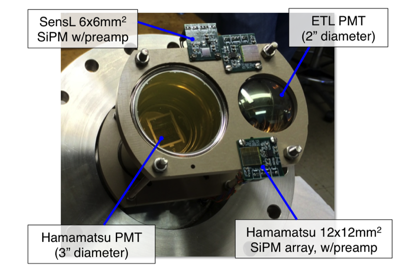
\includegraphics[height=2.2in]{Chapter-3/Images/lightsys_pmts.png}
\hspace{1cm}
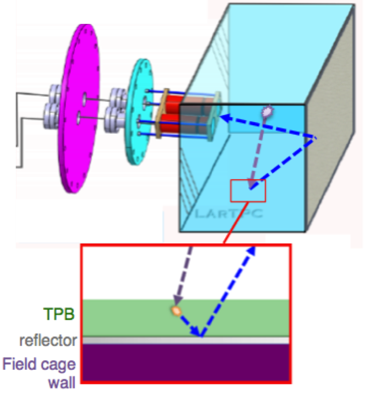
\includegraphics[height=2.2in]{Chapter-3/Images/lightsys_wls.png}
\caption{LArIAT's photodetector system for observing LAr scintillation light inside the TPC (left), and a simplified schematic of VUV light being wavelength-shifting along the TPB-coated reflecting foils (right).}
\label{lightsys_pmts}
\end{figure}

Liquid argon scintillates in vacuum-ultraviolet (VUV) range at 128 nm; since cryogenic PMTs are not sensitive to VUV wavelengths, we need to shift the light to a range that is visible to the PMTs. In LArIAT, the wavelength shifting is achieved by installing highly-reflective 3M VIKUITI dielectric substrate foils coated with a thin layer of tetraphenyl-butadiene (TPB) on the four unbiased walls of the TPC. The scintillation light interaction with the TPB emits one or more visible photons, which are then reflected into the chamber. Thus, the light yield increases and results in higher uniformity of light across the TPC active volume, allowing the possibility of light-based calorimetry, currently under study.

For Run II, we coated   the windows of the ETL PMT and the SensL SiPM  with a thin layer of TPB. In doing so, some of the VUV scintillation light converts into visible right at the sensor faces, keeping information on the direction of the light source. Information about the light directionality is hindered for the light reflected on foils, as the reflection is uniform in angle. %For Run-II, the voltage dividers for the PMTs were configured for positive bias with a DC-coupled anode (AC-coupled anode with grounded photocathode) to minimize induced noise on the TPC wires and modify the PMT bases accordingly.  



\section{Trigger and DAQ}
The LArIAT DAQ and trigger system governs the read out of all the many subsystems forming LArIAT. 
The CAEN V1495 module \cite{CAEN1495} and its user-programmable FPGA  are the core of this system.  Every 10~ns, this module checks for matches between sixteen logical inputs and user-defined patterns in the trigger menu; if it finds a match for two consecutive clock ticks, that trigger fires.

LArIAT receives three logic signals from the Fermilab accelerator complex related to the beam timing which we use as input triggers: a pulse just  before the beam, a pulse indicating beam-on, and a beam-off pulse.

The beam instruments,  the cosmic ray taggers, and the light collection system provide the other NIM-standard logic pulse inputs to the trigger decision. We automatically log the trigger inputs configuration with the rest of the DAQ configuration at the beginning of each run.

Fundamental inputs to the trigger card come from the TOF (see Section~\ref{sec:TOF}) and the wire chambers (see Section~\ref{sec:MWPC}), as activity in these systems points to the presence of a charged particle in tertiary beam line.
In particular, the discriminated pulses from the TOF PMTs form a NIM logic pulse for the trigger logic. We ask for a coincidence within a 20~ns window for all the pulses from the PMTs looking at the same scintillator block and use a delayed coincidence between the upstream and downstream paddle to inform the trigger decision. In order to form a coincidence between the upstream and downstream paddles, we delay the upstream paddle coincidence by 20~ns and widen it by 100~ns. The delay and widening are necessary to account for both  lightspeed particles and slower particles (high-mass) to travel the 6.5~m between the upstream and the downstream paddles. 
For the read out of the wire chambers, we use a total of sixteen multi-hit TDCs\cite{Sten}, four per chamber: two TDC per plane (horizontal and vertical), sixty-four wires per TDC. In each TDC, we keep the logical ``OR" for any signal over threshold from the sixty-four wires. We then require a coincidence between the ``OR" for the horizontal TDCs and the ``OR" for the vertical TDCs: with this logic we make sure that at least one horizontal wire and one vertical wire saw significant signal in one wire chamber.  The single logical pulse from each of the four wire chambers feeds into the first four inputs to the V1495 trigger card. We require a coincidence within 20~ns of at least three logical inputs to form a trigger.


The cosmic towers (see Section~\ref{sec:CosmicRayPaddle}) provide another primary input to the trigger, in order to capture long tracks from cosmic muons crossing the TPC. We use NIM modules to require coincidences between one upper and one lower paddle set of any opposite cosmic towers. The OR all the opposite towers' coincidences is fed as an input to the trigger card. 

We use the signal from the cryogenic PMTs (see Section \ref{sec:TPCLight}) to form several interesting triggers. The coincidence of signals from all the PMT pulses within $\sim$20~ns is an indication of ionizing radiation in the TPC and forms a trigger input.  The coincidence of two subsequent scintillation logic pulses delayed by a maximum of  7~$\mu$s forms the Michel electron trigger. 




\section{Control Systems}
LArIAT is a complex ensemble of systems which needed to be monitored simultaneously during data taking.  We performed the monitoring of the systems operations with a slow control system, a DAQ monitoring system and a low level data quality monitoring system described in the following sections.

\subsubsection{Slow Control}
We used the Synoptic Java Web Start framework \cite{Synoptic} as a real-time display of subsystem conditions. Synoptic provides a Graphical User Interface that talks to the Fermilab Accelerator Control System via the ACNET protocol. Its simple GUI allowed us to change the operating parameters and to graph the trends of several variables of interest for all of the tertiary beam detectors.  Among the most important quantities monitored by Synoptic are the level of argon in both the inner vessel and the external dewar, the operating voltages of cathode and wire planes, of the PMTs and SiPMs, and of the four wire chambers, as well as the magnet temperatures. Figure \ref{fig:synoptics} shows an example of the monitoring system.
LArIAT uses the Accelerator Control NETwork system (ACNET) to monitor the beam conditions of the MCenter beamline. For example, the horizontal and vertical position of the beam at the first two wire chambers (WC1 and WC2) are shown in \ref{fig:ACNET} as seen by the shifter during data taking. 

\begin{figure}[htb]
\centering
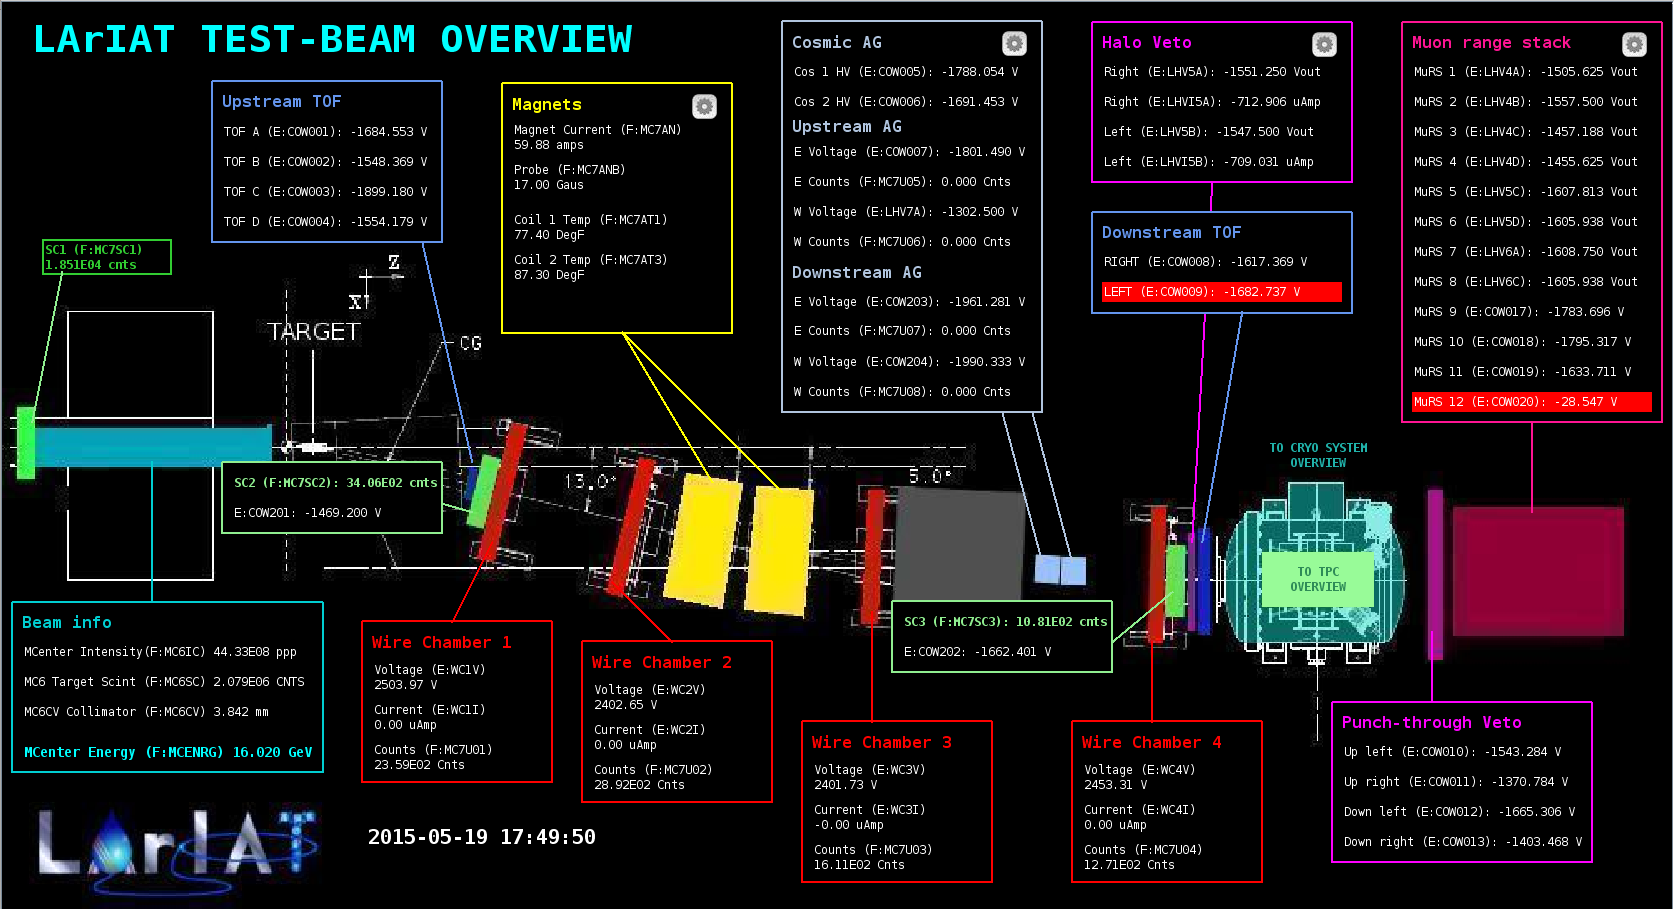
\includegraphics[width=\textwidth,height=\textheight,keepaspectratio]{Chapter-3/Images/BeamOverview.png}
\caption{Interface of the Synoptic slow control system}
\label{fig:synoptics}
\end{figure}

\begin{figure}[htb]
\centering
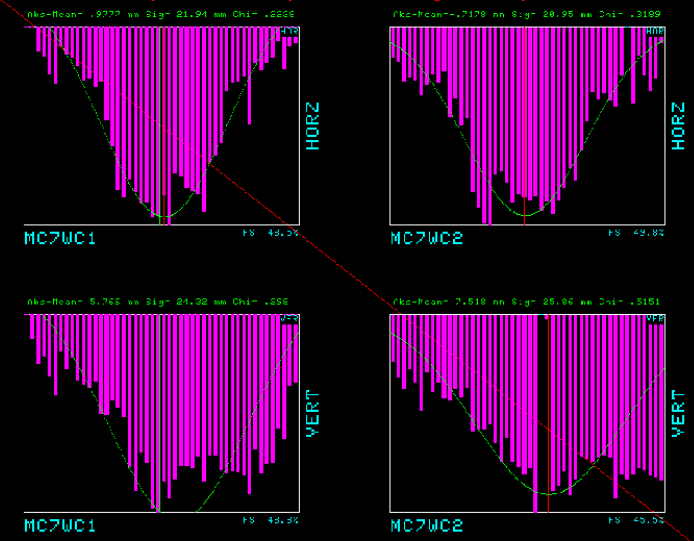
\includegraphics[scale=0.5]{Chapter-3/Images/BeamPosition.png}
\caption{Beam position at the upstream wire chambers monitored with ACNET.}
\label{fig:ACNET}
\end{figure}

\subsubsection{DAQ Monitoring}

We monitor the data taking and the run time evolution with the Run Status Webpage (\href{http://lariat-wbm.fnal.gov/lariat/run.html}{http://lariat-wbm.fnal.gov/lariat/run.html}), a  webpage updated in real-time.  The page displays, among other information, the total number of triggers in the event, the total number of detectors triggered during a beam spill,  the trigger patterns, the number of times a particular trigger pattern was satisfied  during a beam spill, and the current time relative to the Fermilab accelerator complex supercycle. A screen shot of the page is show in figure \ref{fig:runcond}.

\begin{figure}[htb]
\centering
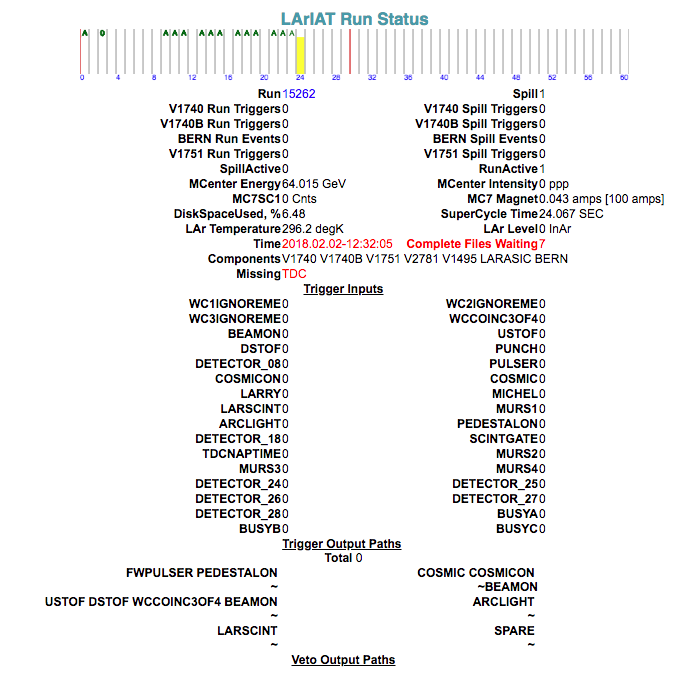
\includegraphics[scale=0.6]{Chapter-3/Images/RunConditions.png}
\caption{Run Status page at LArIAT downtime. At the top the yellow bar displays the current position in the Fermilab supercycle. Interesting information to be monitored by the shifter were the run number and number of spills, time elapsed from data taking (here in red), the energy of the secondary beam and the trigger paths.}
\label{fig:runcond}
\end{figure}



\subsubsection{Data Quality Monitoring}
We employ two systems to ensure the quality of our data during data taking: the Near-Real-Time Data Quality Monitoring and the Event Viewer.

\href{http://lariat-daq01.fnal.gov:5000/}{The Near-Real-Time Data Quality Monitoring} (DQM) is a  webpage which receives updates from all the VME boards in the trigger system and displays the results of a quick analysis of the DAQ stream of raw data on a spill-by-spill basis. The DQM allows the shifter to monitor almost in real time (typically with a 2-minute delay)  a series of low level-quantities and compare them to past collections of beam spills. Some of the variables monitored in the DQM are  the pedestal mean and RMS on CAEN digitizer boards
of the TPC wires and PMTs of the beamline detectors, the hit occupancy and timing plots on the wire chambers, and number of data fragments recorded that are used to build a TPC event. Abnormal values for  low-level quantity in the data  activates a series of alarms in the DQM; this quick feedback on the DAQ and beam conditions is fundamental to assure a fast debugging of the detector and a very efficient data taking during beam uptime.

The online Event Viewer displays a two dimensional representation (Wire vs Time) of LArIAT TPC events  on both the Induction and the Collection planes in near real time. The raw pulses collected by the DAQ on each wire are plotted as a function of drift time, resulting in an image of the TPC event easily readable by the shifter. This tool guarantees a particularly good  check of the TPC operation which activate an immediate feedback for troubleshooting a number of issues. For example,  it is easy for the shifter to spot high occupancy events and request a reduction of the primary beam intensity, or to spot a decrease of the argon purity which requires the regeneration of filters, or to catch the presence of electronic noise and reboot the ASICs. An example of high occupancy event is shown in \ref{fig:highOcc}.

\begin{figure}[htb]
\centering
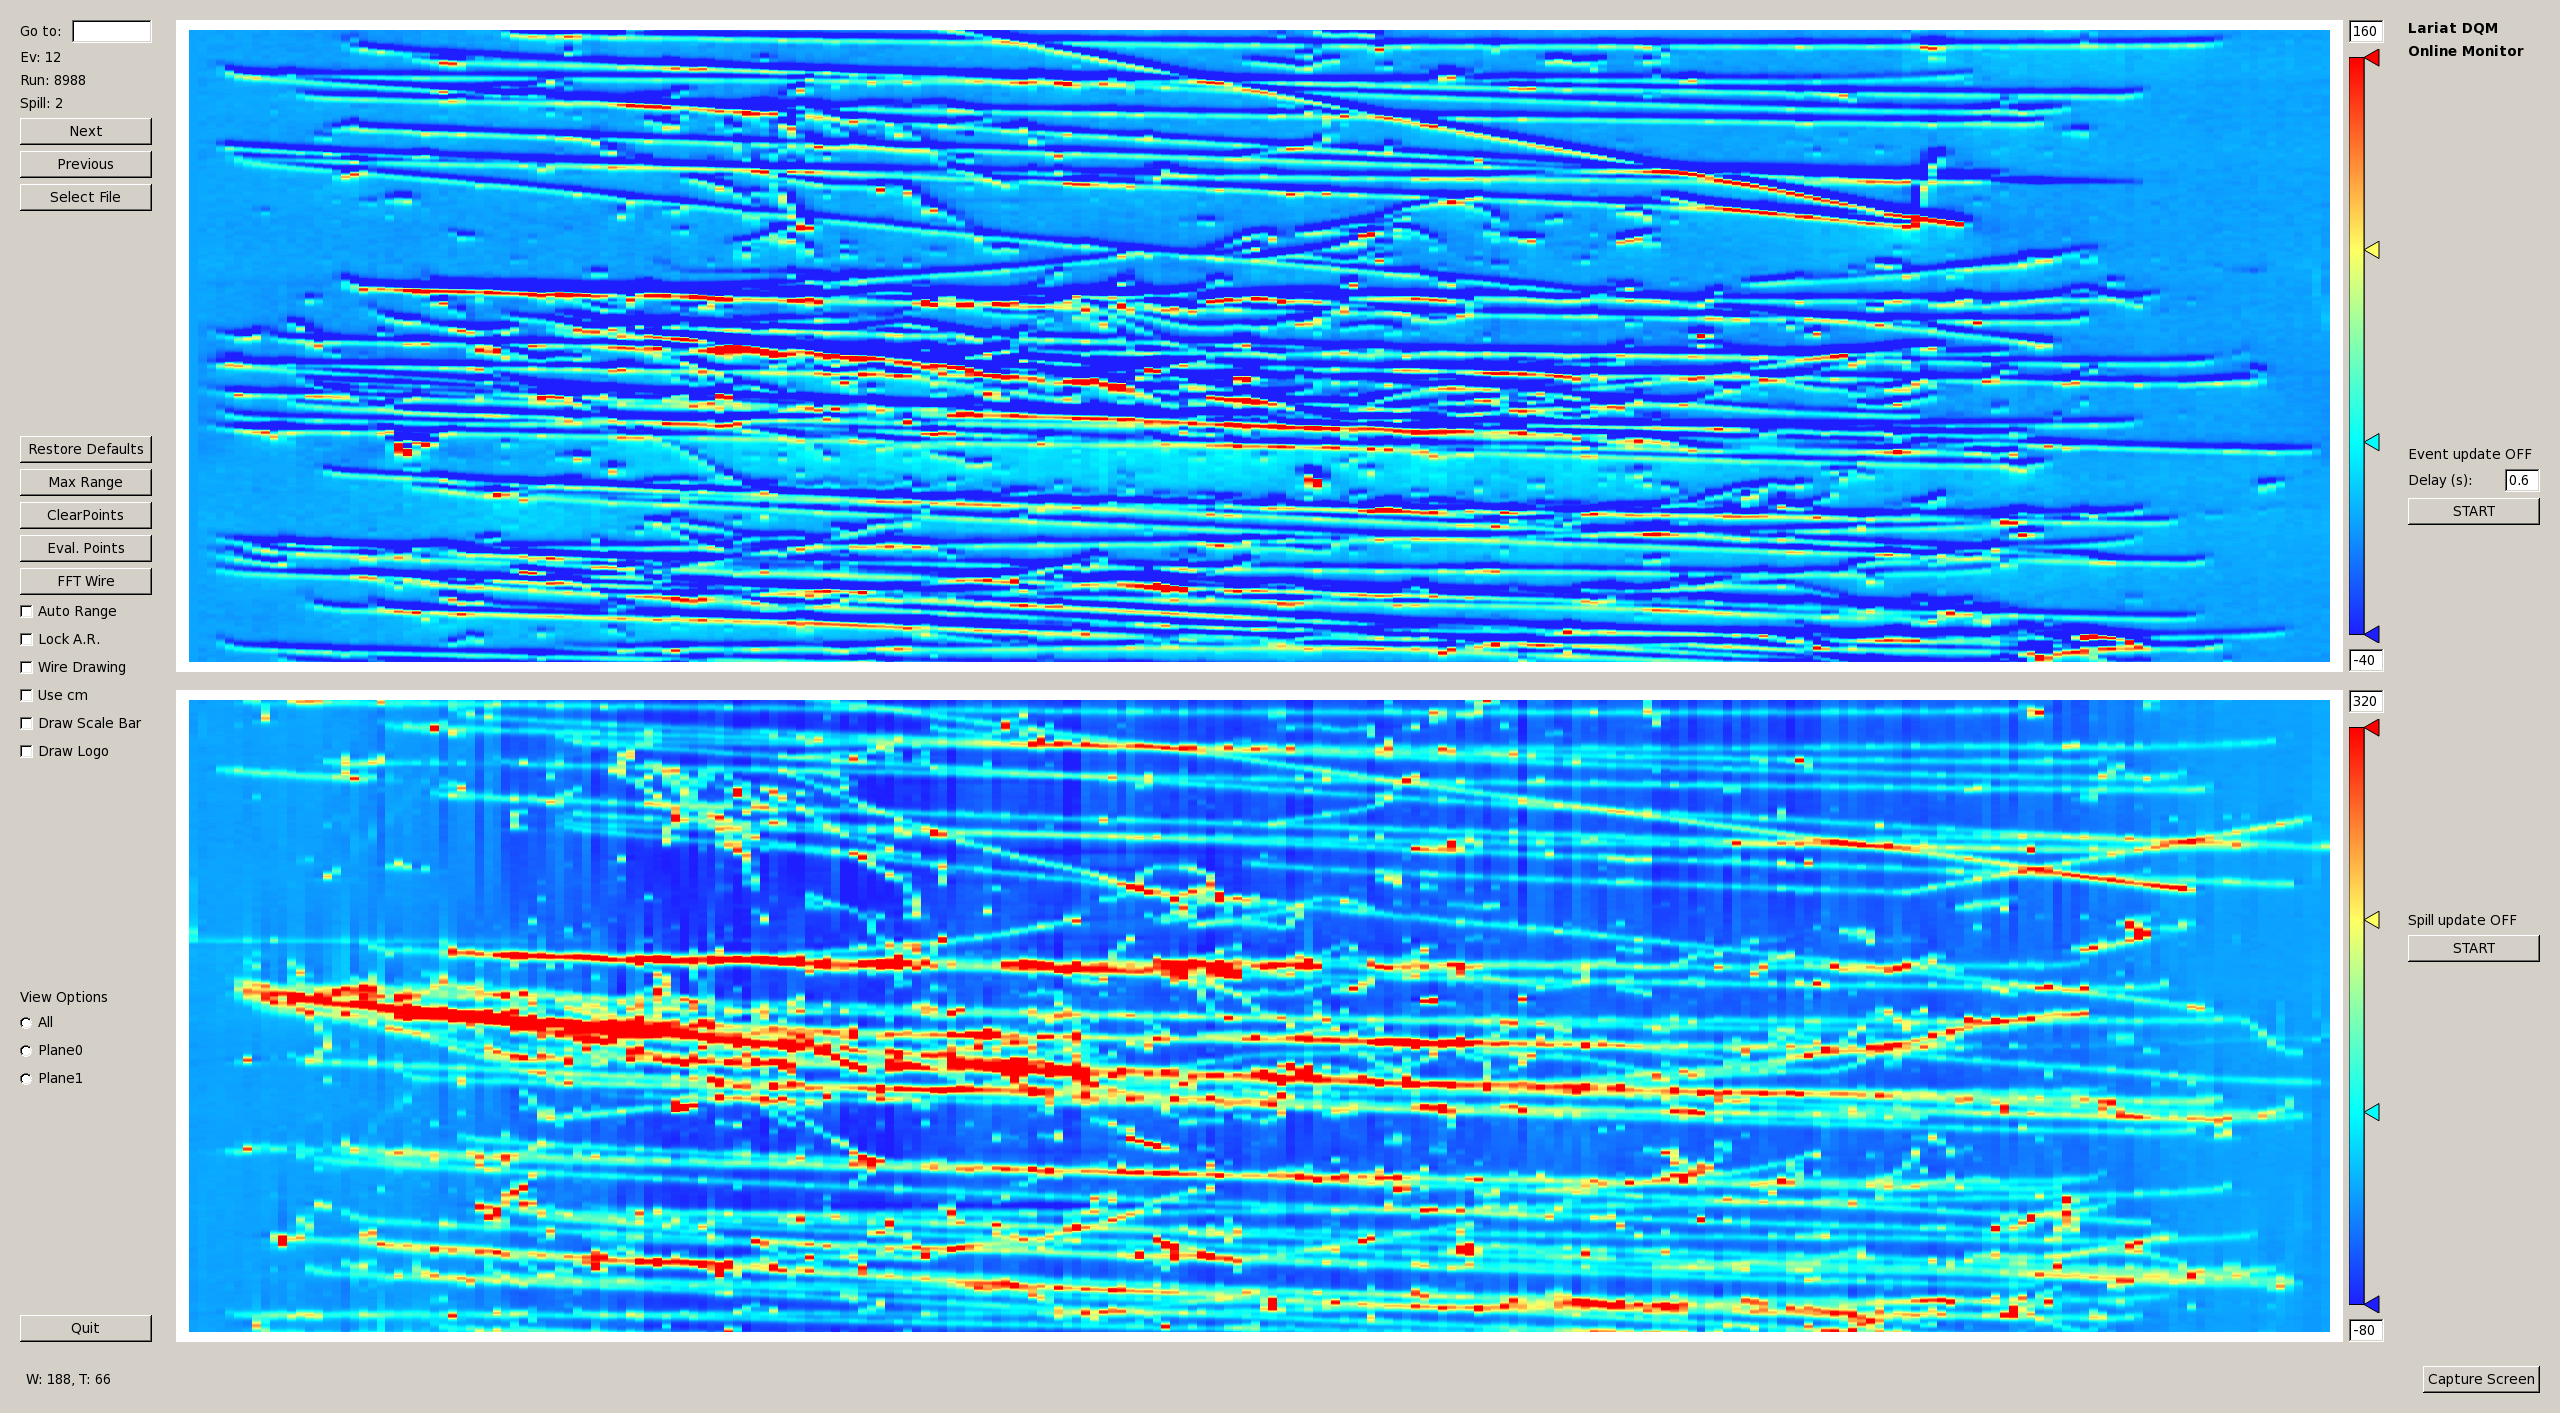
\includegraphics[scale=0.2]{Chapter-3/Images/highOccupancy.png}
\caption{High occupancy event display: induction plane (top) and collection plane (bottom).}
\label{fig:highOcc}
\end{figure}


